\chapter{Espectros electrónicos y magnetismo de los complejos}\label{ch:b3:complex-spectra-magnetism}

El rubí es rojo y la esmeralda es verde, y sin embargo ambos deben su color al mismo ion,
\ce{Cr^{3+}}, que sustituye a unos pocos iones de aluminio en dos óxidos distintos: el corindón,
$\ce{Al2O3}$, en el rubí, y el berilo, un silicato de berilio y aluminio, en la esmeralda. En
ambos, el cromo ocupa un octaedro de átomos de oxígeno; en el berilo el
octaedro es algo mayor y el campo de ligandos algo más débil, y las
bandas de absorción del ion se desplazan unos mil números de onda hacia el rojo.
Eso basta para que el color transmitido pase del rojo al verde. Este capítulo
explica esos espectros cuantitativamente: cómo se desdoblan los términos de un ion libre en un
campo de ligandos, cómo los \omterm{def:b3:complex-spectra-magnetism:tanabe-sugano}{diagramas de Tanabe--Sugano} convierten la posición de dos bandas en el
desdoblamiento del campo de ligandos y la repulsión electrónica, por qué unas bandas son intensas
y otras débiles, por qué algunos complejos se distorsionan y cómo el magnetismo cuenta los
electrones desapareados.

\begin{recall}
El volumen del segundo año trató los elementos de transición y sus configuraciones $d^n$, el
desdoblamiento del campo cristalino $\Delta_{\mathrm o}$, los complejos de alto y bajo espín, la energía de apareamiento,
la energía de estabilización del campo cristalino, las transiciones $d$--$d$, la serie espectroquímica,
la teoría del campo de ligandos y las sustancias paramagnéticas y diamagnéticas.
El \cref{ch:b3:many-electron-atoms} dedujo los \omterm{def:b3:many-electron-atoms:term}{símbolos de término} y las reglas de Hund;
el \cref{ch:b3:group-theory-applied} redujo representaciones y \omterm{def:b3:group-theory-applied:direct-product}{productos directos};
el \cref{ch:b3:electronic-spectroscopy} enunció las reglas de selección de espín y de Laporte
y describió las \omterm{def:b3:electronic-spectroscopy:charge-transfer}{transiciones de transferencia de carga}, y
el \cref{ch:b3:partition-functions} dio la \omterm{def:b3:partition-functions:boltzmann}{distribución de Boltzmann}.
\end{recall}

\begin{omfigure}
\begin{minipage}[b]{0.3\linewidth}\centering
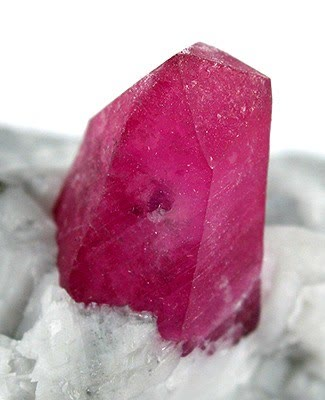
\includegraphics[height=4.2cm]{images/book4/ruby-crystal.jpg}\par
{\small rubí}
\end{minipage}\hspace{1.5em}
\begin{minipage}[b]{0.3\linewidth}\centering
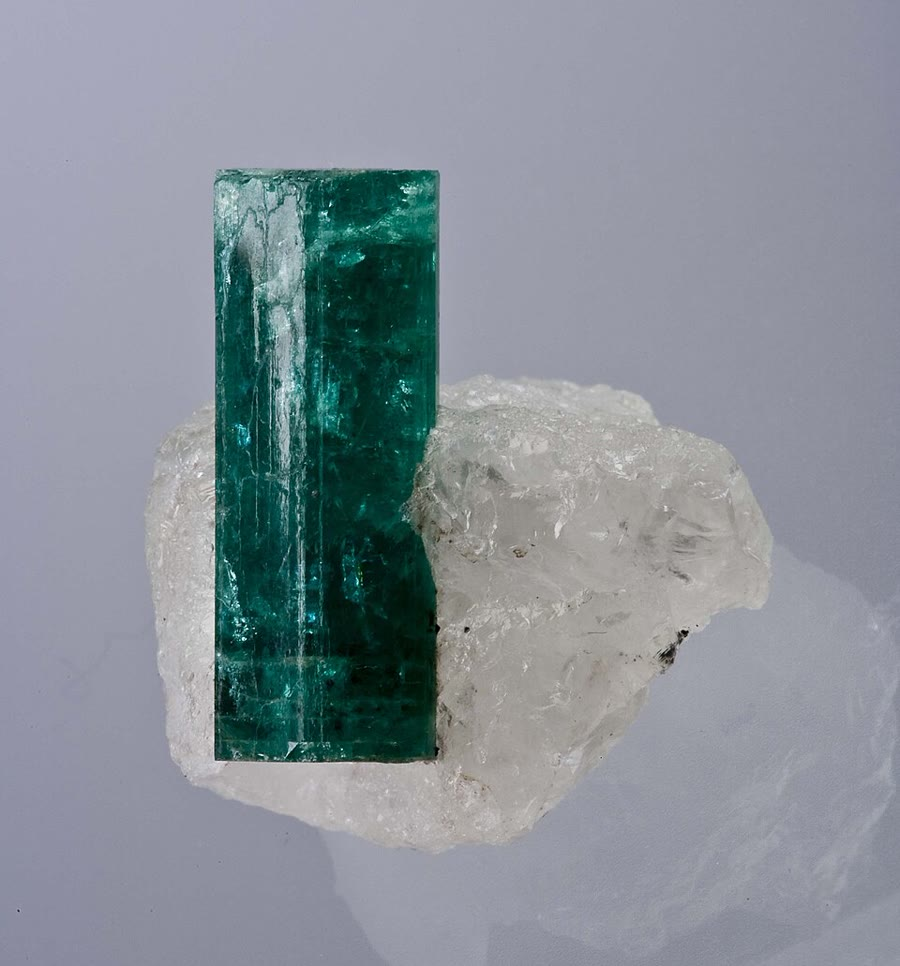
\includegraphics[height=4.2cm]{images/book4/emerald-crystal.jpg}\par
{\small esmeralda}
\end{minipage}

{\small Un cristal de rubí en mármol y un cristal de esmeralda sobre cuarzo. En ambos, el
color se debe a unos pocos por ciento de \ce{Cr^{3+}} en un sitio octaédrico.}
\end{omfigure}

\section{De los términos del ion libre a los términos del campo de ligandos}

En un ion libre, la repulsión electrónica desdobla una configuración $d^n$ en términos
($^4$F, $^4$P, $^2$G\dots\ para $d^3$, \cref{ch:b3:many-electron-atoms}). En un complejo, cada término
se desdobla además por efecto de los ligandos, y los niveles se etiquetan con las \omterm{def:b3:point-groups:irrep}{representaciones
irreducibles} del \omterm{def:b3:point-groups:point-group}{grupo puntual} del complejo.

\begin{definition}[Término del campo de ligandos]\label{def:b3:complex-spectra-magnetism:ligand-field-term}
Un \emph{término del campo de ligandos}\index{termino del campo de ligandos@término del campo de ligandos} de un complejo es un conjunto de
estados polielectrónicos degenerados etiquetado por su \omterm{def:b3:many-electron-atoms:term}{multiplicidad de espín} y por la
\omterm{def:b3:point-groups:irrep}{representación irreducible} del \omterm{def:b3:point-groups:point-group}{grupo puntual} a la que pertenece su parte
orbital, como $^4$A$_{2g}$ o $^4$T$_{1g}$ en un complejo octaédrico.
\end{definition}

\begin{proposition}[Caracteres del grupo de rotaciones]\label{prop:b3:complex-spectra-magnetism:rotation-characters}
Los $2L+1$ estados de un término de momento angular orbital $L$ forman una representación
de las rotaciones cuyo \omterm{def:b3:point-groups:representation}{carácter} para una rotación de ángulo $\alpha$ es
\[
  \chi_L(\alpha) = \frac{\sin\bigl((L + \tfrac12)\alpha\bigr)}{\sin(\alpha/2)}, \qquad \chi_L(0) = 2L + 1 .
\]
\end{proposition}

\admitted

\begin{theorem}[Desdoblamiento de los términos del ion libre en un campo octaédrico]\label{thm:b3:complex-spectra-magnetism:term-splitting}
En un campo octaédrico, los términos de un ion $d^n$ se desdoblan en
\begin{center}
\begin{tabular}{ll}
\hline
término del ion libre & términos octaédricos (misma \omterm{def:b3:many-electron-atoms:term}{multiplicidad de espín}) \\ \hline
S & A$_{1g}$ \\
P & T$_{1g}$ \\
D & E$_g$ + T$_{2g}$ \\
F & A$_{2g}$ + T$_{1g}$ + T$_{2g}$ \\
G & A$_{1g}$ + E$_g$ + T$_{1g}$ + T$_{2g}$ \\ \hline
\end{tabular}
\end{center}
\end{theorem}

\begin{proof}
El grupo octaédrico es el grupo de rotaciones $O$ por la inversión; las funciones $d$
son pares, de modo que todo término de una configuración $d^n$ es par ($g$), y basta con
reducir en $O$, cuyas clases son $E$, $8C_3$, $3C_2$ ($=C_4^2$), $6C_4$ y $6C_2'$. Con la
proposición, para $L = 3$: $\chi = 7$, $\sin(420^\circ)/\sin60^\circ = 1$, $\sin(630^\circ)/\sin90^\circ = -1$, $\sin(315^\circ)/\sin45^\circ = -1$
y $-1$. La \omterm{def:b3:point-groups:irrep}{tabla de caracteres} de $O$ (filas $A_1$: 1, 1, 1, 1, 1; $A_2$: 1, 1, 1, $-1$, $-1$; $E$: 2,
$-1$, 2, 0, 0; $T_1$: 3, 0, $-1$, 1, $-1$; $T_2$: 3, 0, $-1$, $-1$, 1) y la \omterm{thm:b3:group-theory-applied:reduction}{fórmula de reducción} del
\cref{ch:b3:group-theory-applied} dan $n(A_2) = (7 + 8 - 3 + 6 + 6)/24 = 1$, $n(T_1) = (21 + 3 - 6 +
6)/24 = 1$, $n(T_2) = (21 + 3 + 6 - 6)/24 = 1$, y cero para $A_1$ y $E$. Las demás filas se
obtienen del mismo modo ($L = 0$: $(1, 1, 1, 1, 1)$; $L = 1$: $(3, 0, -1, 1, -1)$; $L = 2$: $(5, -1, 1,
-1, 1)$; $L = 4$: $(9, 0, 1, 1, 1)$).
\end{proof}

\begin{method}[Desdoblar un término del ion libre]\label{met:b3:complex-spectra-magnetism:split-term}
\begin{enumerate}
  \item Encontrar el término fundamental del ion libre (reglas de Hund) y los términos
        excitados de la misma multiplicidad.
  \item Leer sus componentes octaédricas en la tabla; la \omterm{def:b3:many-electron-atoms:term}{multiplicidad de espín} no
        cambia.
  \item Ordenarlas: para el término fundamental F de $d^2$ y $d^7$ (alto espín), la más baja es T$_{1g}$;
        para $d^3$ y $d^8$, es A$_{2g}$ (proposición siguiente).
\end{enumerate}
\end{method}

\begin{proposition}[Huecos e inversión tetraédrica]\label{prop:b3:complex-spectra-magnetism:hole}
Los términos de $d^{10-n}$ en un campo octaédrico son los de $d^n$ en orden de energía
inverso; los términos de $d^n$ en un campo tetraédrico son los de $d^{10-n}$ en un campo
octaédrico (sin los subíndices $g$).
\end{proposition}

\begin{proof}
Una configuración $d^{10-n}$ equivale a $n$ huecos positivos en una capa llena: los
huecos sienten el potencial del campo de ligandos con el signo opuesto, de modo que todo
desdoblamiento monoelectrónico, y por tanto todo desdoblamiento de términos, se invierte (la
repulsión electrónica entre huecos es la misma que entre electrones). Un campo
tetraédrico tiene el signo opuesto al de uno octaédrico (los orbitales $e$
quedan más bajos) y no tiene centro de simetría: $d^n$ en $T_d$ se comporta como $d^n$ con un campo
invertido, es decir, como $d^{10-n}$ en $O_h$.
\end{proof}

\begin{definition}[Diagrama de correlación]\label{def:b3:complex-spectra-magnetism:correlation}
Un \emph{diagrama de correlación}\index{diagrama de correlacion@diagrama de correlación} une los estados de un
sistema en dos situaciones límite, aquí los términos del ion libre desdoblados por un campo
débil y las configuraciones $t_{2g}^ae_g^b$ de un campo fuerte, conectando estados de la
misma simetría sin dejar que dos de ellos se crucen.
\end{definition}

\begin{omfigure}
\begin{tikzpicture}[font=\small]
  % free ion
  \pic (F) at (0,0) {omlevel={}{1.1}};
  \pic (P) at (0,3.0) {omlevel={}{1.1}};
  \node[anchor=east] at (F-l) {$^3$F};
  \node[anchor=east] at (P-l) {$^3$P};
  % weak field
  \pic (a) at (2.6,-0.8) {omlevel={}{1.0}};
  \pic (b) at (2.6,0.3) {omlevel={}{1.0}};
  \pic (c) at (2.6,1.4) {omlevel={}{1.0}};
  \pic (d) at (2.6,3.1) {omlevel={}{1.0}};
  \foreach \n/\t in {a/T$_{1g}$, b/T$_{2g}$, c/A$_{2g}$, d/T$_{1g}$(P)}{\node[omsymlabel, anchor=south] at (\n-c) {$^3$\t};}
  \draw[omcorr] (F-r) -- (a-l) (F-r) -- (b-l) (F-r) -- (c-l) (P-r) -- (d-l);
  % strong field configurations
  \pic (A) at (7.4,-1.6) {omlevel={}{1.0}};
  \pic (B) at (7.4,1.4) {omlevel={}{1.0}};
  \pic (C) at (7.4,1.9) {omlevel={}{1.0}};
  \pic (D) at (7.4,4.6) {omlevel={}{1.0}};
  \node[anchor=west] at (A-r) {$^3$T$_{1g}$ \quad $t_{2g}^2$};
  \node[anchor=west] at (B-r) {$^3$T$_{2g}$};
  \node[anchor=west] at (C-r) {$^3$T$_{1g}$ \quad $t_{2g}e_g$};
  \node[anchor=west] at (D-r) {$^3$A$_{2g}$ \quad $e_g^2$};
  \draw[omcorr] (a-r) -- (A-l) (b-r) -- (B-l) (c-r) -- (D-l) (d-r) -- (C-l);
  \node[anchor=north] at (0,-2.0) {ion libre};
  \node[anchor=north] at (2.6,-2.0) {campo débil};
  \node[anchor=north] at (7.4,-2.0) {campo fuerte};
  \draw[->, black!50] (3.7,-2.3) -- (6.2,-2.3) node[midway, below, font=\scriptsize] {$\Delta_{\mathrm o}$ creciente};
\end{tikzpicture}

{\small \omterm{def:b3:complex-spectra-magnetism:correlation}{Diagrama de correlación} de los \omterm{def:b3:many-electron-atoms:singlet-triplet}{estados triplete} de un ion $d^2$ en un campo
octaédrico. Cada término de campo débil va a la configuración de campo fuerte de la misma
simetría, y los dos estados $^3$T$_{1g}$ no se cruzan: el inferior va a $t_{2g}^2$, y el superior, a
$t_{2g}e_g$.}
\end{omfigure}

\section{Diagramas de Tanabe--Sugano}

\begin{definition}[Parámetros de Racah]\label{def:b3:complex-spectra-magnetism:racah}
Los \emph{parámetros de Racah}\index{parametros de Racah@parámetros de Racah} $A$, $B$ y $C$ son combinaciones de
las integrales de Slater de la capa $d$ que expresan todas las energías de repulsión
electrónica de una configuración $d^n$; las diferencias de energía entre términos de la
misma configuración solo dependen de $B$ y $C$, y las diferencias entre términos de la misma
multiplicidad máxima, solo de $B$ (para $d^2$, $d^3$, $d^7$, $d^8$: $E(\mathrm P) - E(\mathrm F) = 15B$).
\end{definition}

\begin{example}[Parámetros de Racah del ion libre]\label{ex:b3:complex-spectra-magnetism:free-B}
% ledger: lev:Cr3.4F5_2, lev:Cr3.4F7_2, lev:Cr3.4F9_2, lev:Cr3.4P1_2, lev:Cr3.4P3_2, lev:Cr3.4P5_2, lev:Ni2.3F3, lev:Ni2.3F2, lev:Ni2.3P2, lev:Ni2.3P1, lev:Ni2.3P0, lev:V2.4F5_2, lev:V2.4F7_2, lev:V2.4F9_2, lev:V2.4P1_2, lev:V2.4P3_2, lev:V2.4P5_2
Los niveles del ion \ce{Cr^{3+}} libre sitúan el centro de gravedad (pesos $2J + 1$) de $^4$F a
\qty{547}{cm^{-1}} y el de $^4$P a \qty{14305}{cm^{-1}} por encima del nivel fundamental: $15B = \qty{13758}{cm^{-1}}$,
$B = \qty{917}{cm^{-1}}$. El mismo cálculo da $B = 755$ para \ce{V^{2+}} y \qty{1056}{cm^{-1}} para
\ce{Ni^{2+}}.
\end{example}

\begin{definition}[Diagrama de Tanabe--Sugano]\label{def:b3:complex-spectra-magnetism:tanabe-sugano}
Un \emph{diagrama de Tanabe--Sugano}\index{diagrama de Tanabe--Sugano} representa las energías de
todos los \omterm{def:b3:complex-spectra-magnetism:ligand-field-term}{términos del campo de ligandos} de un ion $d^n$, en unidades de $B$ y medidas desde el
término fundamental, en función de $\Delta_{\mathrm o}/B$, para una razón $C/B$ fija.
\end{definition}

\begin{proposition}[Las tres bandas de un ion $d^3$]\label{prop:b3:complex-spectra-magnetism:d3-bands}
Para un ion $d^3$ en un campo octaédrico, las transiciones permitidas por el espín desde $^4$A$_{2g}$ están en
\[
  \nu_1 = \Delta_{\mathrm o}\ (^4\mathrm T_{2g}), \qquad
  \nu_{2,3} = 7.5B + 1.5\Delta_{\mathrm o} \mp \tfrac12\sqrt{225B^2 - 18B\Delta_{\mathrm o} + \Delta_{\mathrm o}^2}\ (^4\mathrm T_{1g}(\mathrm F), {}^4\mathrm T_{1g}(\mathrm P)).
\]
\end{proposition}

\begin{proof}[Demostración parcial]
En la base de campo fuerte, $^4$A$_{2g}$ y $^4$T$_{2g}$ aparecen una vez cada uno, a partir de $t_{2g}^3$ y de $t_{2g}^2e_g$, y
su diferencia no contiene repulsión electrónica: $\nu_1 = \Delta_{\mathrm o}$ exactamente. $^4$T$_{1g}$ aparece
dos veces, a partir de $t_{2g}^2e_g$ y de $t_{2g}e_g^2$; respecto de $^4$A$_{2g}$, la matriz $2\times2$ es
$\begin{pmatrix}\Delta_{\mathrm o} + 12B & 6B\\ 6B & 2\Delta_{\mathrm o} + 3B\end{pmatrix}$ (los elementos de repulsión electrónica se admiten).
Sus \omterm{def:b3:quantum-model-systems:operator}{valores propios} son las raíces de $E^2 - (15B + 3\Delta_{\mathrm o})E + 2\Delta_{\mathrm o}^2 + 27B\Delta_{\mathrm o} = 0$, que son los
$\nu_2$ y $\nu_3$ enunciados. En $\Delta_{\mathrm o} = 0$ valen 0 y $15B$ (los términos $^4$F y $^4$P); la
diagonalización completa de la figura los reproduce.
\end{proof}

\begin{omfigure}
\begin{tikzpicture}
\begin{axis}[name=ta, omts, width=0.46\linewidth, height=7.0cm, xmin=1, xmax=40, ymin=0, ymax=70,
  xlabel={$\Delta_{\mathrm o}/B$}, ylabel={$E/B$}, title={\small $d^3$, $C/B = 4.5$},
  unbounded coords=jump, clip=true, clip mode=individual]
\foreach \c in {f0,f1,f2,f3,f4,f5,f6,f7,f8,f9,f10,f11,f12,f13,f14,f15}{
  \addplot[omtsforbidden, restrict x to domain=1:40] table[x=x, y=\c] {figdata/out/bachelor-3-tanabe-sugano-d3.dat};}
\foreach \c in {a0,a1,a2,a3}{
  \addplot[omDef, thick, restrict x to domain=1:40] table[x=x, y=\c] {figdata/out/bachelor-3-tanabe-sugano-d3.dat};}
\draw[omThm, dashed] (axis cs:29.0,0) -- (axis cs:29.0,70);
\draw[black!70, dashed] (axis cs:27.1,0) -- (axis cs:27.1,70);
\node[font=\scriptsize, omThm, anchor=north west, rotate=90] at (axis cs:29.6,1.5) {rubí};
\node[font=\scriptsize, anchor=south west, rotate=90] at (axis cs:26.6,1.5) {esmeralda};
% labels outside the frame, at the height where each curve leaves it
\node[font=\scriptsize, omDef, anchor=west, inner sep=1pt] at (axis cs:40,40) {$^4$T$_{2g}$};
\node[font=\scriptsize, omDef, anchor=west, inner sep=1pt] at (axis cs:40,50.9) {$^4$T$_{1g}$};
\node[font=\scriptsize, omDef, anchor=south, inner sep=1pt] at (axis cs:32.8,70) {$^4$T$_{1g}$(P)};
\node[font=\scriptsize, black!60, anchor=west, inner sep=1pt] at (axis cs:40,21.2) {$^2$E$_g$};
\end{axis}
\begin{axis}[at={(ta.east)}, anchor=west, xshift=2.2cm, omts, width=0.46\linewidth, height=7.0cm,
  xmin=1, xmax=40, ymin=0, ymax=70, xlabel={$\Delta_{\mathrm o}/B$}, ylabel={$E/B$},
  title={\small $d^8$, $C/B = 4.71$}, unbounded coords=jump, clip=true, clip mode=individual]
\foreach \c in {f0,f1,f2,f3,f4,f5,f6}{
  \addplot[omtsforbidden, restrict x to domain=1:40] table[x=x, y=\c] {figdata/out/bachelor-3-tanabe-sugano-d8.dat};}
\foreach \c in {a0,a1,a2,a3}{
  \addplot[omDef, thick, restrict x to domain=1:40] table[x=x, y=\c] {figdata/out/bachelor-3-tanabe-sugano-d8.dat};}
\node[font=\scriptsize, omDef, anchor=west, inner sep=1pt] at (axis cs:40,40) {$^3$T$_{2g}$};
\node[font=\scriptsize, omDef, anchor=west, inner sep=1pt] at (axis cs:40,50.9) {$^3$T$_{1g}$};
\node[font=\scriptsize, omDef, anchor=south, inner sep=1pt] at (axis cs:32.8,70) {$^3$T$_{1g}$(P)};
\end{axis}
\end{tikzpicture}

{\small \omterm{def:b3:complex-spectra-magnetism:tanabe-sugano}{Diagramas de Tanabe--Sugano} de iones $d^3$ y $d^8$ calculados diagonalizando el
hamiltoniano de campo de ligandos y de repulsión electrónica sobre todos los estados de la
configuración. En azul grueso: los estados de la multiplicidad del estado fundamental
(transiciones permitidas por el espín); en gris fino: los demás. El término fundamental es el
eje horizontal ($^4$A$_{2g}$ para $d^3$, $^3$A$_{2g}$ para $d^8$). En trazo discontinuo: el rubí y la esmeralda, situados en el $\Delta_{\mathrm o}/B$ de sus dos bandas.
El nivel $^2$E$_g$ de $d^3$ es casi plano: su energía apenas depende del campo.}
\end{omfigure}

\begin{method}[Leer un diagrama de Tanabe--Sugano]\label{met:b3:complex-spectra-magnetism:read-ts}
\begin{enumerate}
  \item Identificar el término fundamental y las transiciones permitidas por el espín (misma
        multiplicidad).
  \item Calcular la razón de las energías de dos bandas, $\nu_2/\nu_1$; encontrar el valor de $\Delta_{\mathrm o}/B$ en
        el que el diagrama da esa razón.
  \item Leer allí $E/B$ para $\nu_1$: $B = \nu_1/(E/B)$, y después $\Delta_{\mathrm o}$. Para $d^3$ y $d^8$, $\Delta_{\mathrm o} = \nu_1$
        directamente, y la fórmula cerrada da $B$ a partir de $\nu_2$.
  \item Comparar $B$ con el valor del ion libre (\omterm{def:b3:complex-spectra-magnetism:nephelauxetic}{razón nefelauxética}) y comprobar que la
        tercera banda cae donde el diagrama predice.
\end{enumerate}
\end{method}

\begin{definition}[Efecto nefelauxético]\label{def:b3:complex-spectra-magnetism:nephelauxetic}
El \emph{efecto nefelauxético}\index{efecto nefelauxetico@efecto nefelauxético} (``que expande la nube'') es
la disminución del parámetro de Racah $B$ de un ion metálico en un complejo respecto del
ion libre, causada por la deslocalización de los electrones $d$ hacia los
ligandos; la \emph{razón nefelauxética}\index{razon nefelauxetica@razón nefelauxética} es $\beta =
B_{\text{complejo}}/B_{\text{ion libre}}$.
\end{definition}

Los ligandos que se enlazan de forma más covalente reducen más $B$: $\beta$ vale cerca de 0.9 para el fluoruro, 0.8
para el agua, de 0.6 a 0.7 para el óxido y los haluros más pesados, y menos aún para el sulfuro.
Las transiciones prohibidas por el espín, entre términos de distinta multiplicidad, aparecen
como rayas débiles, a menudo estrechas.

\section{Intensidades y transferencia de carga}

\begin{definition}[Acoplamiento vibrónico]\label{def:b3:complex-spectra-magnetism:vibronic-coupling}
El \emph{acoplamiento vibrónico}\index{acoplamiento vibronico@acoplamiento vibrónico} es la mezcla de los movimientos
electrónico y de vibración: una vibración asimétrica que elimina el centro de
simetría de un complejo mezcla un poco de carácter impar ($u$) en sus estados $d$,
lo que hace débilmente permitidas las transiciones $d$--$d$ prohibidas por la \omterm{thm:b3:electronic-spectroscopy:laporte}{regla de Laporte}.
\end{definition}

\begin{proposition}[Intensidades de las bandas de absorción]\label{prop:b3:complex-spectra-magnetism:intensity-order}
Los coeficientes de absorción molar de las bandas de los complejos aumentan en el
orden: $d$--$d$ prohibida por el espín $\ll$ $d$--$d$ permitida por el espín en un complejo centrosimétrico $<$ $d$--$d$
en un complejo tetraédrico $<$ transferencia de carga.
\end{proposition}

\begin{proof}[Argumento]
Según el \cref{ch:b3:electronic-spectroscopy}, una transición está permitida cuando se conserva el
espín y cambia la paridad. Una transición $d$--$d$ nunca cambia la paridad: en un complejo
octaédrico solo toma prestada intensidad mediante el \omterm{def:b3:complex-spectra-magnetism:vibronic-coupling}{acoplamiento vibrónico}; en un
tetraedro, que no tiene centro, los orbitales $d$ y $p$ se mezclan de forma permanente. Una
transición prohibida por el espín toma prestada además una pequeña fracción mediante el \omterm{def:b3:many-electron-atoms:spin-orbit}{acoplamiento
espín--órbita}. Una \omterm{def:b3:electronic-spectroscopy:charge-transfer}{transición de transferencia de carga} lleva un electrón entre orbitales de
distinta paridad del metal y del ligando, y está plenamente permitida.
\end{proof}

\begin{definition}[Transferencia de carga]\label{def:b3:complex-spectra-magnetism:ct}
En una \emph{transferencia de carga del ligando al metal}\index{transferencia de carga del ligando al metal}
(LMCT), un electrón pasa de un orbital centrado en el ligando a uno centrado en el
metal; en una \emph{transferencia de carga del metal al ligando}\index{transferencia de carga del metal al ligando}
(MLCT), del metal a un orbital $\pi^*$ de un ligando.
\end{definition}

El permanganato y el cromato, iones $d^0$ sin ninguna transición $d$--$d$, deben sus intensos
colores a una LMCT del óxido hacia un orbital $d$ vacío del metal, fácil para un metal en un estado
de oxidación alto. El $\ce{[Ru(bpy)3]^{2+}}$ (bpy: 2,2$'$-bipiridina) debe su color naranja a una MLCT
del rutenio(II) hacia los orbitales $\pi^*$ de los ligandos, el estado excitado que se usa en la
\omterm{def:b3:photochemistry:photoredox}{catálisis fotorredox} (\cref{ch:b3:photochemistry}). En el rubí, las dos bandas anchas
hacia 560 y \qty{410}{nm} son las bandas $d$--$d$ permitidas por el espín de la
\cref{prop:b3:complex-spectra-magnetism:d3-bands}; la luz que pasa es roja,
con algo de azul. Excitado en estas bandas, el ion se relaja al nivel $^2$E$_g$ y
emite desde él la raya R, de un rojo intenso, hacia \qty{695}{nm}, la raya del primer láser.

\section{El efecto Jahn--Teller}

\begin{theorem}[Teorema de Jahn--Teller]\label{thm:b3:complex-spectra-magnetism:jahn-teller}
Una molécula no lineal en un estado electrónico orbitalmente degenerado es inestable
frente a una distorsión que rebaja su simetría y levanta la
\omterm{def:b3:quantum-model-systems:degenerate}{degeneración}. Es el \emph{teorema de Jahn--Teller}\index{teorema de Jahn--Teller}.
\end{theorem}

\admitted

Sus consecuencias para los complejos octaédricos se deducen de la ocupación de los
orbitales $e_g$, que apuntan hacia los ligandos. En un ion $d^9$ (\ce{Cu^{2+}}), la configuración
$t_{2g}^6e_g^3$ tiene el hueco en $d_{z^2}$ o en $d_{x^2-y^2}$: un estado E$_g$. Alargar los dos enlaces
axiales baja $d_{z^2}$ y sube $d_{x^2-y^2}$; poner dos electrones en el orbital que baja
y uno en el que sube da una estabilización neta. Los complejos de cobre(II) son
en efecto octaedros alargados, con cuatro enlaces cortos y dos largos. Lo mismo vale
para $d^4$ de alto espín (\ce{Mn^{3+}}, \ce{Cr^{2+}}) y $d^7$ de bajo espín; para los conjuntos $t_{2g}$ llenos de forma desigual
($d^1$, $d^2$, $d^5$ de bajo espín\dots), los orbitales apuntan entre los ligandos y la
distorsión es pequeña. Los estados excitados degenerados de los complejos también se distorsionan: las
bandas anchas, a menudo con dos jorobas, del \ce{[Ti(H2O)6]^{3+}} y de los complejos de cobre(II) son
la firma espectroscópica de ello.

\begin{omfigure}
\begin{tikzpicture}[font=\small]
  \pic[transform shape] (t) at (0,0) {omlevel={}{1.6}};
  \pic[transform shape] (e) at (0,2.2) {omlevel={}{1.1}};
  \node[anchor=east] at (t-l) {$t_{2g}$};
  \node[anchor=east] at (e-l) {$e_g$};
  \pic[transform shape] (xy) at (4.2,0.45) {omlevel={ud}{0.8}};
  \pic[transform shape] (xz) at (4.2,-0.25) {omlevel={ud}{1.4}};
  \pic[transform shape] (x2) at (4.2,3.0) {omlevel={u}{0.8}};
  \pic[transform shape] (z2) at (4.2,1.5) {omlevel={ud}{0.8}};
  \draw[omcorr] (t-r) -- (xy-l) (t-r) -- (xz-l) (e-r) -- (x2-l) (e-r) -- (z2-l);
  \node[anchor=west] at (xy-r) {$b_{2g}$ ($d_{xy}$)};
  \node[anchor=west] at (xz-r) {$e_g$ ($d_{xz}$, $d_{yz}$)};
  \node[anchor=west] at (x2-r) {$b_{1g}$ ($d_{x^2-y^2}$)};
  \node[anchor=west] at (z2-r) {$a_{1g}$ ($d_{z^2}$)};
  \node[anchor=north] at (0,-0.9) {$O_h$};
  \node[anchor=north] at (4.2,-0.9) {$D_{4h}$, alargado};
  \begin{scope}[xshift=9.0cm, yshift=1.2cm, scale=0.8]
    \pic[transform shape] {omoctahedron};
    \draw[->, thick, omThm] (0,1.25) -- (0,1.85);
    \draw[->, thick, omThm] (0,-1.25) -- (0,-1.85);
  \end{scope}
\end{tikzpicture}

{\small Distorsión de Jahn--Teller de un complejo octaédrico $d^9$: alargar los enlaces axiales (derecha) desdobla $e_g$ en $a_{1g}$
($d_{z^2}$, que baja) y $b_{1g}$ ($d_{x^2-y^2}$, que sube), y $t_{2g}$ en $e_g$ y $b_{2g}$. Con nueve
electrones, el único hueco está en $b_{1g}$: la distorsión es una estabilización neta.}
\end{omfigure}

\section{Magnetismo}

\begin{definition}[Susceptibilidad magnética]\label{def:b3:complex-spectra-magnetism:susceptibility}
La \emph{susceptibilidad magnética}\index{susceptibilidad magnetica@susceptibilidad magnética} $\chi$ de un material
es la razón entre su imanación y la intensidad del campo aplicado; la \emph{susceptibilidad
molar}\index{susceptibilidad molar} $\chi_{\mathrm m}$ es la susceptibilidad por mol.
Las sustancias paramagnéticas tienen $\chi > 0$; las diamagnéticas, una $\chi < 0$ pequeña. Los químicos suelen
usar el valor cgs de $\chi_{\mathrm m}$, en \unit{cm^3.mol^{-1}}, igual al valor SI en \unit{m^3.mol^{-1}}
dividido por $4\pi\times10^{-6}$.
\end{definition}

\begin{definition}[Constante de Curie]\label{def:b3:complex-spectra-magnetism:curie}
La \emph{constante de Curie}\index{constante de Curie} $C$ de un paramagneto que obedece a la
\omterm{thm:b3:complex-spectra-magnetism:curie}{ley de Curie} es el producto $\chi_{\mathrm m}T$.
\end{definition}

\begin{theorem}[Ley de Curie]\label{thm:b3:complex-spectra-magnetism:curie}
Para espines independientes $S$ cuyo factor $g$ vale $g$, a temperaturas a las que $g\mu_BB \ll kT$,
\[
  \chi_{\mathrm m} = \frac{C}{T}, \qquad C = \frac{\mu_0N_Ag^2\mu_B^2S(S+1)}{3k}\ \ (\text{SI});
\]
en unidades cgs, $C = 0.1251\,g^2S(S+1)$ \unit{cm^3.K.mol^{-1}}. Es la \emph{ley de Curie}\index{ley de Curie}.
\end{theorem}

\begin{proof}[Demostración parcial]
Para $S = \frac12$, los dos niveles $m_S = \pm\frac12$ tienen las energías $\pm\frac12g\mu_BB$ en un campo $B$. Según la
\omterm{def:b3:partition-functions:boltzmann}{distribución de Boltzmann}, el momento medio en la dirección del campo es $\frac12g\mu_B\tanh(g\mu_BB/2kT) \approx
g^2\mu_B^2B/4kT$; por mol, $M = N_Ag^2\mu_B^2B/4kT$, y con $\chi_{\mathrm m} = \mu_0M/B$, $\chi_{\mathrm m} = \mu_0N_Ag^2\mu_B^2/(4kT)$,
que es la fórmula con $S(S+1) = \frac34$. El caso general (promediando $m_S^2$ sobre $2S + 1$
niveles, $\langle m_S^2\rangle = S(S+1)/3$) se admite.
\end{proof}

\begin{definition}[Momento magnético efectivo]\label{def:b3:complex-spectra-magnetism:moment}
El \emph{momento magnético efectivo}\index{momento magnetico efectivo@momento magnético efectivo} de un
ion paramagnético es $\mu_{\mathrm{eff}} = \sqrt{3k\chi_{\mathrm m}T/(\mu_0N_A)}$, en cgs $\mu_{\mathrm{eff}}/\mu_B = 2.828\sqrt{\chi_{\mathrm m}T}$. Su
\emph{momento de solo espín}\index{momento de solo espin@momento de solo espín} es el valor $2\sqrt{S(S+1)}\,\mu_B$ que darían
los espines por sí solos con $g = 2$; el exceso del momento medido sobre él es
la \emph{contribución orbital}\index{contribucion orbital@contribución orbital}.
\end{definition}

\begin{proposition}[Fórmula de solo espín]\label{prop:b3:complex-spectra-magnetism:spin-only}
Para $n$ electrones desapareados, $\mu_{\text{solo espín}} = \sqrt{n(n+2)}\,\mu_B$: 1.73, 2.83, 3.87, 4.90 y $5.92\,\mu_B$ para
$n = 1$ a 5.
\end{proposition}

\begin{proof}
$S = n/2$, luego $2\sqrt{S(S+1)} = 2\sqrt{\frac n2(\frac n2 + 1)} = \sqrt{n(n+2)}$.
\end{proof}

\begin{proposition}[Contribuciones orbitales]\label{prop:b3:complex-spectra-magnetism:orbital-contribution}
En un complejo octaédrico, los iones con términos fundamentales A o E tienen momentos próximos al
valor de solo espín; los iones con términos fundamentales T pueden tener \omterm{def:b3:complex-spectra-magnetism:moment}{contribuciones orbitales}
importantes.
\end{proposition}

\begin{proof}[Argumento]
Un momento orbital necesita un orbital que pueda transformarse en otro equivalente y
degenerado mediante una rotación en torno al eje del campo, con un electrón libre de
moverse entre ellos. En un estado T (conjunto $t_{2g}$ lleno de forma desigual), los orbitales $d_{xz}$, $d_{yz}$, $d_{xy}$
están relacionados por rotaciones de $90^\circ$ y el momento sobrevive en parte; en los estados A y E
($t_{2g}^3$, $t_{2g}^6e_g^2$, $e_g$ parcialmente lleno) no hay ningún orbital equivalente disponible y el
momento orbital está extinguido.
\end{proof}

\begin{definition}[Transición de espín]\label{def:b3:complex-spectra-magnetism:spin-crossover}
La \emph{transición de espín}\index{transicion de espin@transición de espín} es la conversión de un complejo entre
un estado de bajo espín y uno de alto espín por efecto de la temperatura, la presión o la luz, posible
cuando $\Delta_{\mathrm o}$ está próximo a la energía de apareamiento.
\end{definition}

\begin{proposition}[Temperatura de transición]\label{prop:b3:complex-spectra-magnetism:crossover}
Si la conversión $\mathrm{LS} \rightleftharpoons \mathrm{HS}$ se comporta como un equilibrio de entalpía $\Delta H$ y entropía $\Delta S$, la
fracción de alto espín es $x_{\mathrm{HS}} = 1/(1 + \eu^{(\Delta H - T\Delta S)/RT})$, igual a un medio en $T_{1/2} = \Delta H/\Delta S$.
\end{proposition}

\begin{proof}
$K = x_{\mathrm{HS}}/(1 - x_{\mathrm{HS}}) = \eu^{-(\Delta H - T\Delta S)/RT}$; $K = 1$ cuando $\Delta H = T\Delta S$.
\end{proof}

Tanto $\Delta H$ como $\Delta S$ son positivas: el estado de alto espín tiene enlaces metal--ligando más largos
y más débiles y más estados de espín ($R\ln5$ solo por el espín para el hierro(II), $S = 2$), de modo que se impone a
alta temperatura.

\begin{omfigure}
\begin{tikzpicture}
\begin{axis}[name=ct, width=0.47\linewidth, height=5.2cm, xmin=0, xmax=400, ymin=0, ymax=5.6,
  axis lines=left, xlabel={$T$ / K}, ylabel={$\chi_{\mathrm m}T$ / \unit{cm^3.K.mol^{-1}}},
  tick label style={font=\small}, label style={font=\small}]
\addplot[omDef, thick] table[x=T, y=chiT_para] {figdata/out/bachelor-3-curie-chiT.dat};
\addplot[omThm, thick] table[x=T, y=chiT_sco] {figdata/out/bachelor-3-curie-chiT.dat};
\node[font=\scriptsize, omDef, anchor=south west] at (axis cs:20,4.45) {paramagneto de Curie, $S = \frac52$};
\node[font=\scriptsize, omThm, anchor=west, align=left] at (axis cs:20,2.4) {transición de espín,\\ $T_{1/2} = \qty{200}{K}$};
\end{axis}
\begin{axis}[at={(ct.east)}, anchor=west, xshift=1.5cm, width=0.47\linewidth, height=5.2cm,
  xmin=0, xmax=100, ymin=0, ymax=0.46, axis lines=left, xlabel={$1000\,\mathrm K/T$},
  ylabel={$\chi_{\mathrm m}$ / \unit{cm^3.mol^{-1}}}, tick label style={font=\small},
  label style={font=\small}]
\addplot[omDef, thick] table[x=invT, y=chi] {figdata/out/bachelor-3-curie-chi.dat};
\end{axis}
\end{tikzpicture}

{\small Izquierda: $\chi_{\mathrm m}T$ en función de $T$ para un paramagneto de Curie ($S = \frac52$, $g = 2$: constante,
\qty{4.38}{cm^3.K.mol^{-1}}) y para un compuesto modelo de hierro(II) con \omterm{def:b3:complex-spectra-magnetism:spin-crossover}{transición de espín} ($\Delta H =
\qty{15}{kJ/mol}$, $\Delta S = \qty{75}{J.K^{-1}.mol^{-1}}$), que pasa de 0 (bajo espín, $S = 0$) a
\qty{3.0}{cm^3.K.mol^{-1}} (alto espín, $S = 2$). Derecha: la \omterm{thm:b3:complex-spectra-magnetism:curie}{ley de Curie}, $\chi_{\mathrm m}$ lineal en $1/T$.}
\end{omfigure}

\begin{definition}[Magnetismo cooperativo]\label{def:b3:complex-spectra-magnetism:cooperative}
En el \emph{ferromagnetismo}\index{ferromagnetismo}, los espines de centros paramagnéticos
vecinos se alinean paralelamente mediante una interacción de intercambio, lo que da una
imanación espontánea por debajo de la temperatura de Curie; en el
\emph{antiferromagnetismo}\index{antiferromagnetismo} se alinean antiparalelamente, y
la susceptibilidad disminuye por debajo de la temperatura de Néel.
\end{definition}

En los complejos dinucleares, el mismo acoplamiento de intercambio aparece como un $\chi_{\mathrm m}T$ que disminuye
(antiferromagnético) o aumenta (ferromagnético) al enfriar, a partir del cual se ajusta la constante
de acoplamiento; los ligandos puente como el óxido o el acetato suelen acoplar los
metales de forma antiferromagnética.

\begin{method}[El momento magnético por el método de Evans]\label{met:b3:complex-spectra-magnetism:evans}
\begin{enumerate}
  \item En un tubo de RMN, poner la disolución del compuesto paramagnético (de concentración
        conocida $c$) con un poco de una referencia inerte (terc-butanol, la señal residual del
        disolvente); en un tubo interior coaxial, el mismo disolvente y la
        referencia sin el compuesto.
  \item Registrar el espectro de \ce{^1H}: la referencia da dos rayas separadas $\Delta f$.
  \item En un imán superconductor (campo según el tubo), la diferencia de susceptibilidad
        volúmica es $\Delta\chi_v = 3\Delta f/f$ (SI, se admite); $\chi_{\mathrm m} = \Delta\chi_v/c$ ($c$ en
        \unit{mol.m^{-3}}), corregida del diamagnetismo del compuesto si es necesario;
        y después $\mu_{\mathrm{eff}}$.
\end{enumerate}
\end{method}

\begin{inthelab}[Una medida de Evans]
Un capilar sellado a la llama, o un inserto coaxial comercial, contiene el disolvente de
referencia dentro del tubo de RMN. La medida lleva un minuto en cualquier espectrómetro
de rutina; los errores principales proceden de la concentración y de la
temperatura, que debe conocerse, ya que $\chi_{\mathrm m}$ varía como $1/T$.
\end{inthelab}

\begin{safety}{\ghs[0.56cm]{GHS03}\ghs[0.56cm]{GHS05}\ghs[0.56cm]{GHS06}\ghs[0.56cm]{GHS07}\ghs[0.56cm]{GHS08}\ghs[0.56cm]{GHS09}}
% ledger: ghs:K2Cr2O7
Dicromato de potasio y cromatos usados para los espectros de transferencia de carga:
comburentes, tóxicos, pueden provocar cáncer y defectos genéticos hereditarios, muy tóxicos para
los organismos acuáticos. Se pesan en un recinto ventilado con guantes; los residuos de cromo(VI)
se reducen y se recogen por separado.
\end{safety}

\begin{history}[Jahn y Teller, Tanabe y Sugano]
Hermann Jahn y Edward Teller demostraron en 1937, examinando todos los \omterm{def:b3:point-groups:point-group}{grupos puntuales},
que la \omterm{def:b3:quantum-model-systems:degenerate}{degeneración} orbital y un armazón nuclear simétrico son incompatibles en las
moléculas no lineales. Yukito Tanabe y Satoru Sugano calcularon en 1954 las
energías de todos los términos de los iones $d^2$ a $d^8$ en campos octaédricos,
diagonalizando las mismas matrices que la figura de este capítulo; sus
diagramas se han usado desde entonces para asignar los espectros de los complejos.
\end{history}

\section{Ejercicios}

\begin{exercise}[$\star$]\label{exo:b3:complex-spectra-magnetism:1}
Dense las componentes octaédricas de los términos D, F y G, y compruébese que las
\omterm{def:b3:quantum-model-systems:degenerate}{degeneraciones} suman $2L + 1$.
\end{exercise}

\begin{exercise}[$\star$]\label{exo:b3:complex-spectra-magnetism:2}
Para $d^1$ a $d^9$ (alto espín), dense el término fundamental del ion libre y el término octaédrico del que
pasa a ser el estado fundamental.
\end{exercise}

\begin{exercise}[$\star$]\label{exo:b3:complex-spectra-magnetism:3}
Calcúlense los \omterm{def:b3:complex-spectra-magnetism:moment}{momentos de solo espín} de \ce{Mn^{2+}}, \ce{Fe^{2+}} y \ce{Co^{2+}} de alto espín, y de
\ce{Fe^{2+}} y \ce{Co^{3+}} de bajo espín.
\end{exercise}

\begin{exercise}[$\star$]\label{exo:b3:complex-spectra-magnetism:4}
Ordénense por intensidad creciente las bandas visibles de \ce{MnO4-}, $\ce{[Mn(H2O)6]^{2+}}$, $\ce{[CoCl4]^{2-}}$ y
$\ce{[Co(H2O)6]^{2+}}$, y justifíquese.
\end{exercise}

\begin{exercise}[$\star\star$]\label{exo:b3:complex-spectra-magnetism:5}
% ledger: lev:Ni2.3F3, lev:Ni2.3F2, lev:Ni2.3P2, lev:Ni2.3P1, lev:Ni2.3P0
Un complejo hexaacuoníquel(II) presenta bandas a 8500, 14100 y \qty{24900}{cm^{-1}} (datos del
ejercicio). Asígnense y, usando $\nu_2 + \nu_3 = 15B + 3\Delta_{\mathrm o}$ (la traza de la matriz de $^3$T$_{1g}$),
encuéntrense $\Delta_{\mathrm o}$, $B$ y $\beta$ (ion libre: $B = \qty{1056}{cm^{-1}}$).
\end{exercise}

\begin{exercise}[$\star\star$]\label{exo:b3:complex-spectra-magnetism:6}
% ledger: lev:Cr3.4F5_2, lev:Cr3.4P5_2
Un complejo hexaacuocromo(III) absorbe a 17400 y \qty{24600}{cm^{-1}} (datos del
ejercicio). Encuéntrense $\Delta_{\mathrm o}$, $B$ y $\beta$, y predígase la tercera banda.
\end{exercise}

\begin{exercise}[$\star\star$]\label{exo:b3:complex-spectra-magnetism:7}
El rubí y la esmeralda tienen \omterm{def:b3:complex-spectra-magnetism:nephelauxetic}{razones nefelauxéticas} de 0.67, y el ion hexaacuocromo(III),
de 0.79. ¿Qué indica esto sobre los enlaces Cr--O en las gemas?
\end{exercise}

\begin{exercise}[$\star\star$]\label{exo:b3:complex-spectra-magnetism:8}
Predígase una distorsión de Jahn--Teller fuerte, débil o nula para $d^9$ octaédrico, $d^4$ de alto
espín, $d^7$ de bajo espín, $d^3$, $d^6$ de alto espín y $d^6$ de bajo espín.
\end{exercise}

\begin{exercise}[$\star\star$]\label{exo:b3:complex-spectra-magnetism:9}
El \ce{Co^{2+}} de alto espín tiene un momento próximo a $5\,\mu_B$ en los complejos octaédricos y más cercano a
$4.4\,\mu_B$ en los tetraédricos (datos del ejercicio). Explíquese a partir de los términos
fundamentales.
\end{exercise}

\begin{exercise}[$\star\star\star$]\label{exo:b3:complex-spectra-magnetism:10}
Un complejo tiene $\chi_{\mathrm m}T = \qty{1.87}{cm^3.K.mol^{-1}}$, independiente de la temperatura. Calcúlense $\mu_{\mathrm{eff}}$ y
el número de electrones desapareados.
\end{exercise}

\begin{exercise}[$\star\star\star$]\label{exo:b3:complex-spectra-magnetism:11}
En una medida de Evans a \qty{400}{MHz} y \qty{298}{K}, una disolución \qty{10.0}{mM} desplaza la
referencia \qty{25.0}{Hz} (datos del ejercicio). Calcúlense $\chi_{\mathrm m}$ (cgs) y $\mu_{\mathrm{eff}}$.
\end{exercise}

\begin{exercise}[$\star\star\star$]\label{exo:b3:complex-spectra-magnetism:12}
Para un compuesto con \omterm{def:b3:complex-spectra-magnetism:spin-crossover}{transición de espín} de $\Delta H = \qty{15}{kJ/mol}$ y $\Delta S = \qty{75}{J.K^{-1}.mol^{-1}}$, calcúlense $T_{1/2}$,
la fracción de alto espín a \qty{250}{K} y el valor de $\chi_{\mathrm m}T$ a esa temperatura (alto espín, $S = 2$).
\end{exercise}

\section{Problema: un ion, dos gemas}

\begin{problem}[{Problema de fin de semana --- un ion, dos gemas: los términos del
cromo(III), las bandas del rubí y de la esmeralda sobre el diagrama $d^3$, el campo de
ligandos y la repulsión electrónica de cada una, y la estrecha raya roja del rubí}]
\label{pb:b3:complex-spectra-magnetism:1}
% ledger: lf:ruby.nu1, lf:ruby.nu2, lf:emerald.nu1, lf:emerald.nu2, lf:ruby.Rline, lev:Cr3.4F5_2, lev:Cr3.4F7_2, lev:Cr3.4F9_2, lev:Cr3.4P1_2, lev:Cr3.4P3_2, lev:Cr3.4P5_2
Máximos de absorción (luz polarizada perpendicularmente al eje del cristal): rubí,
17\,820 y \qty{24170}{cm^{-1}}; esmeralda, 16\,740 y \qty{23040}{cm^{-1}}. El rubí presenta además una
raya estrecha hacia \qty{695}{nm}. \ce{Cr^{3+}} libre: centros de gravedad de $^4$F y $^4$P a 547 y \qty{14305}{cm^{-1}}.

\medskip\noindent\textbf{Parte I --- El cromo(III).}
\begin{enumerate}
  \item Dese la configuración electrónica de \ce{Cr^{3+}}.
  \item Dese su término fundamental de ion libre.
  \item Desdóblese en un campo octaédrico.
  \item ¿Qué componente es el término fundamental, y por qué?
  \item ¿En qué se convierte el término $^4$P?
  \item Enumérense las transiciones permitidas por el espín.
\end{enumerate}

\medskip\noindent\textbf{Parte II --- Las bandas.}
\begin{enumerate}[resume]
  \item Conviértanse las bandas del rubí en longitudes de onda.
  \item Conviértanse las bandas de la esmeralda en longitudes de onda.
  \item Explíquense los dos colores.
  \item Dese el $\Delta_{\mathrm o}$ de cada gema.
  \item ¿Por qué $\nu_1$ es exactamente $\Delta_{\mathrm o}$?
\end{enumerate}

\medskip\noindent\textbf{Parte III --- La repulsión electrónica.}
\begin{enumerate}[resume]
  \item Calcúlese el $B$ del ion libre.
  \item Usando la fórmula de $\nu_2$, encuéntrese $B$ para el rubí (resuélvase numéricamente).
  \item Hágase lo mismo para la esmeralda.
  \item Calcúlense las \omterm{def:b3:complex-spectra-magnetism:nephelauxetic}{razones nefelauxéticas}.
  \item Calcúlese $\Delta_{\mathrm o}/B$ para cada gema y sitúense en el diagrama.
  \item Predígase la tercera banda permitida por el espín del rubí. ¿Por qué rara vez se observa?
  \item Propóngase por qué el campo es más débil en la esmeralda.
\end{enumerate}

\medskip\noindent\textbf{Parte IV --- La raya R.}
\begin{enumerate}[resume]
  \item Calcúlese la energía de la raya a \qty{695}{nm} y su valor en unidades del $B$ del rubí.
  \item El diagrama trazado con $C/B = 4.5$ sitúa $^2$E$_g$ en $21.0B$. ¿Qué indica la diferencia
        sobre la $C/B$ del rubí?
  \item ¿Por qué es estrecha la raya, a diferencia de las bandas anchas?
  \item ¿Por qué es lenta la emisión?
  \item ¿Por qué debería estar la raya casi en la misma posición en la esmeralda?
  \item ¿Por qué un nivel excitado de vida larga hace posible un láser?
  \item Enúnciese el resultado: la diferencia $\Delta_{\mathrm o}(\text{rubí}) - \Delta_{\mathrm o}(\text{esmeralda})$.
\end{enumerate}
\end{problem}
